\documentclass[11pt]{article}
\usepackage[margin=1in]{geometry}
\usepackage{amsmath,amssymb,amsthm,mathtools}
\usepackage{graphicx}
\usepackage[hidelinks]{hyperref}
\usepackage{xcolor}

\newtheorem{theorem}{Theorem}
\newtheorem{lemma}[theorem]{Lemma}
\newtheorem{remark}[theorem]{Remark}
\newcommand{\R}{\mathbb R}
\newcommand{\HS}{\mathcal S_2}
\newcommand{\tr}{\operatorname{tr}}
\setlength{\emergencystretch}{2em}

\title{The Hilbert--Schmidt basis-learning objective\\
need not attain its spectral supremum}
\author{Autonomous mathematical discovery run \texttt{fa\_banach\_001}}
\date{27 August 2026}

\begin{document}
\maketitle

\noindent\textbf{Status.}
Candidate full counterexample to optimizer existence, likely valid pending
expert review.

\section{Source target}

Kamkari, Nabizadeh, and Solomon define $\mathcal{SO}(HS)$ using orthogonal
flows generated by Hilbert--Schmidt skew-adjoint operators
\cite[Definition~1, PDF p.~4]{KNS}.  Their Theorem~2 treats the maximum
\begin{equation}\label{eq:source}
 \max_{Q\in\mathcal{SO}(HS)}
 \sum_{i\geq1}p(i)\langle Q\varphi_i,AQ\varphi_i\rangle
\end{equation}
as having a solution $Q^{\rm opt}$ and concludes that the transformed basis
is an eigenbasis ordered by decreasing eigenvalue
\cite[Theorem~2 and equation~(7), PDF p.~5]{KNS}.

\begin{center}
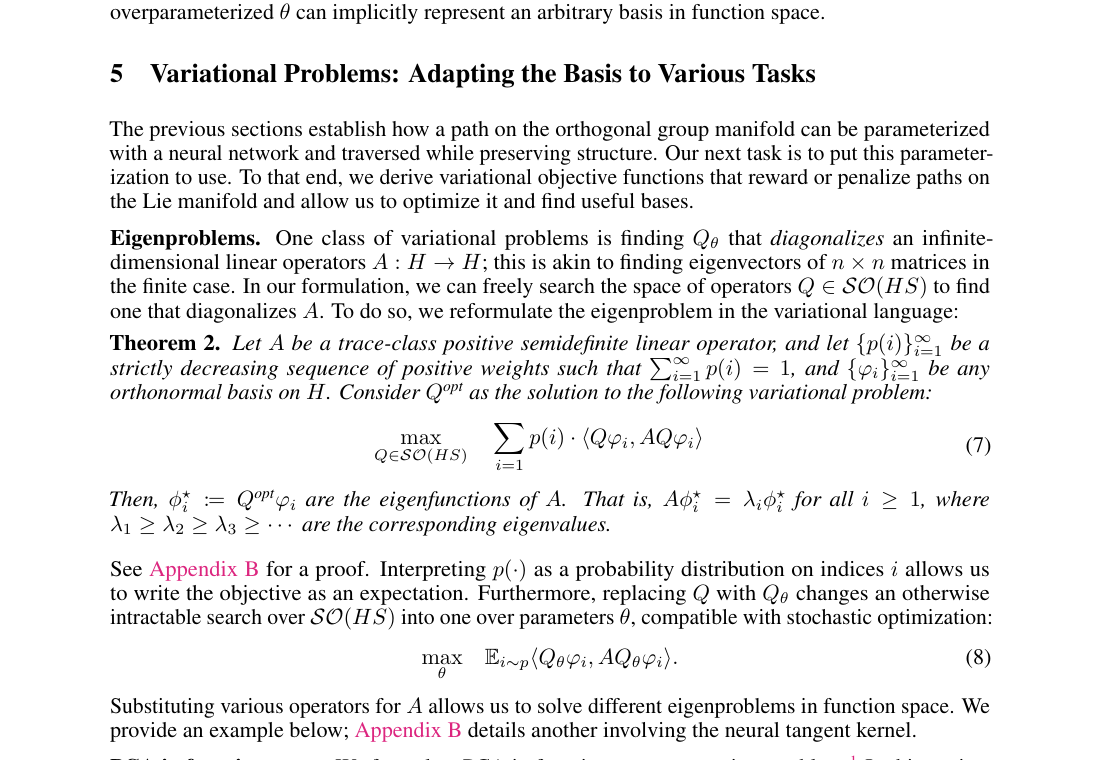
\includegraphics[width=0.91\textwidth]{figures/source_theorem2.png}
\end{center}

The example below shows that the displayed supremum need not be attained.
It lies entirely inside the paper's function-space/PCA setting: the domain is
compact, the reference and target bases consist of continuous functions, and
$A$ is a positive trace-class covariance operator with continuous kernel.

\section{Proof intuition}

Pair the Fourier functions and rotate every pair through $90^\circ$.  Give
the resulting ordered basis the simple eigenvalues $2^{-i}$, and use the same
numbers as the objective weights.  Exact spectral alignment requires moving
\emph{every} reference vector by a fixed distance.  Such a change of basis is
not identity plus Hilbert--Schmidt, hence is outside the source's admissible
class.  Rotating only the first $m$ pairs is admissible and misses the optimum
by exactly $1/(15\cdot16^m)$.  Thus the objective has a maximizing sequence
whose limit has escaped the Hilbert--Schmidt group.

\section{Counterexample and exact value}

Write $u\otimes v$ for the rank-one operator
$f\mapsto\langle f,v\rangle u$.

\begin{theorem}\label{thm:main}
Let $H=L^2([0,1];\R)$ and let $(\varphi_i)_{i\geq1}$ be an enumeration of
the real Fourier orthonormal basis.  There are strictly decreasing positive
weights $p(i)$ summing to one and a positive trace-class operator $A$ with a
continuous integral kernel such that the objective in \eqref{eq:source}
satisfies
\[
 \sup_{Q\in\mathcal{SO}(HS)}
 \sum_{i\geq1}p(i)\langle Q\varphi_i,AQ\varphi_i\rangle
 =\frac13,
\]
but no $Q\in\mathcal{SO}(HS)$ attains $1/3$.
Moreover, admissible finite-rank exponentials $Q_m$ attain exactly
\[
 \frac13-\frac{1}{15\cdot16^m}\qquad(m\geq0).
\]
The operator $A$ is the covariance of a random continuous function.
\end{theorem}

\begin{proof}
Put $b_i=2^{-i}$ and
\[
 B=\sum_{i\geq1}b_i\,\varphi_i\otimes\varphi_i.
\]
Define the orthogonal quarter-turn $R$ blockwise by
\[
 R\varphi_{2k-1}=\varphi_{2k},\qquad
 R\varphi_{2k}=-\varphi_{2k-1}\qquad(k\geq1),
\]
and set $A=RBR^*$.  Then $A$ is positive and trace class, with distinct
eigenvalues $b_i$ and corresponding ordered eigenvectors
$e_i=R\varphi_i$.

The real Fourier functions are continuous and uniformly bounded by
$\sqrt2$.  Hence
\[
 a(x,y)=\sum_{i\geq1}b_i e_i(x)e_i(y)
\]
converges absolutely and uniformly on $[0,1]^2$, so it is a continuous
integral kernel for $A$.  If $(\varepsilon_i)$ are independent Rademacher
signs, then
\[
 X=\sum_{i\geq1}b_i^{1/2}\varepsilon_i e_i
\]
converges uniformly to a continuous random function because
$\sum_i\sqrt{b_i}<\infty$, and $\mathbb E[X\otimes X]=A$.

Choose $p(i)=b_i=2^{-i}$, so $p$ is strictly decreasing and
$\sum_i p(i)=1$.  For an orthogonal $Q$, set $S=R^*Q$.  The objective is
the Hilbert--Schmidt inner product
\begin{align*}
 F(Q)
 &=\tr(BQ^*AQ)
   =\tr(BS^*BS)
   =\langle B,S^*BS\rangle_{\HS}\\
 &\leq \|B\|_{\HS}\,\|S^*BS\|_{\HS}
   =\|B\|_{\HS}^2
   =\sum_{i\geq1}4^{-i}=\frac13.
\end{align*}
Equality in Cauchy--Schwarz forces $S^*BS=B$.  Thus $BS=SB$; since the
eigenvalues of $B$ are simple, there are signs $\epsilon_i\in\{-1,1\}$
such that $S\varphi_i=\epsilon_i\varphi_i$.  Every equality case therefore
has
\[
 Q\varphi_i=\epsilon_i R\varphi_i,
 \qquad
 \|Q\varphi_i-\varphi_i\|^2=2
 \quad(i\geq1).
\]
Consequently $Q-I$ is not Hilbert--Schmidt.

On the other hand, every member of the source's $\mathcal{SO}(HS)$ satisfies
$Q-I\in\HS$.  Indeed, for $Q=e^K$ with Hilbert--Schmidt skew-adjoint $K$,
\[
 e^K-I=\int_0^1 e^{tK}K\,dt\in\HS.
\]
(The same conclusion follows from Duhamel's formula for the broader
time-dependent flows used later in the source.)  Hence no admissible $Q$ can
be an equality case.

It remains to prove that $1/3$ is nevertheless the supremum.  For $m\geq0$
let
\[
 K_m=\frac\pi2\sum_{k=1}^{m}
 \bigl(\varphi_{2k}\otimes\varphi_{2k-1}
       -\varphi_{2k-1}\otimes\varphi_{2k}\bigr),
 \qquad Q_m=e^{K_m}.
\]
Then $K_m$ is finite-rank, Hilbert--Schmidt, and skew-adjoint; $Q_m$ agrees
with $R$ on the first $m$ pairs and is the identity on the remaining pairs.
Thus $Q_m\in\mathcal{SO}(HS)$.  On a tail pair, the two eigenvalues are
swapped, and direct summation gives
\begin{align*}
 F(Q_m)
 &=\sum_{i=1}^{2m}4^{-i}
   +\sum_{k>m}
     \bigl(2^{-(2k-1)}2^{-2k}
          +2^{-2k}2^{-(2k-1)}\bigr)\\
 &=\frac13-\sum_{k>m}16^{-k}
  =\frac13-\frac{1}{15\cdot16^m}.
\end{align*}
These values increase to $1/3$, proving both the supremum formula and its
nonattainment.
\end{proof}

\section{Structural diagnosis and scope}

The obstruction is topological, not spectral.  The weighted objective is
insensitive to changes far out in the basis, whereas the Hilbert--Schmidt
group requires the squared displacements of \emph{all} basis vectors to be
summable.  The sequence $Q_m$ converges strongly to $R$, but
$R-I\notin\HS$; it does not converge to $R$ in Hilbert--Schmidt topology.
This is precisely the escape mechanism that destroys compactness of the
optimization problem.

The result supplies a full negative answer to the implicit optimizer-
existence question in Theorem~2 and to the surrounding claim that one can
freely search the stated class to find a diagonalizer for every admissible
$A$.  It does \emph{not} refute the conditional assertion that, when a
maximizer exists, strict weights order its eigenvectors.  Nor does it rule
out optimization over a larger orthogonal class or under an additional
compatibility assumption ensuring that an ordered eigenbasis differs from
the reference basis by a Hilbert--Schmidt operator.

The source appendix also estimates a Hilbert--Schmidt norm of an orthogonal
operator itself.  In infinite dimension such an operator is never
Hilbert--Schmidt; only differences such as $Q-I$ may be.  The argument above
avoids that issue and uses only the ideal property of $\HS$.

\section{Verification and novelty}

The accompanying exact-arithmetic regression script checks the finite-pair
objective, the closed formula for the defect, and the divergence of the
required squared basis displacement.  It is not needed for the proof.

A bounded search on 27 August 2026 covered all four run indexes, the current
arXiv record, the exact paper title and theorem name, and searches combining
Hilbert--Schmidt orthogonal groups, diagonalization, optimizer existence, and
nonattainment.  The source remains at version~1, and no correction or later
response was found.  Novelty confidence is moderate pending specialist
review.

\paragraph{Human review recommendation.}
Check that the source intends $\mathcal{SO}(HS)$ literally as Definition~1
rather than the full orthogonal group.  Under either the stationary
definition or the later time-dependent Hilbert--Schmidt-flow definition,
the necessary condition $Q-I\in\HS$ used above is immediate.

\begin{thebibliography}{9}
\raggedright
\bibitem{KNS}
H. Kamkari, M. S. Nabizadeh, and J. Solomon,
\emph{Learning Orthonormal Bases for Function Spaces},
arXiv:2605.19959v1 (2026).
\end{thebibliography}

\end{document}
